\documentclass[tikz,border=3pt]{standalone}
\usepackage{fontspec}
\usepackage{amsmath}
\usepackage{xcolor}
\usepackage{tikz}
\usepackage{pgfplots}
\pgfplotsset{compat=1.18}
\usetikzlibrary{arrows.meta,calc,fit,positioning,shapes.geometric,shapes.misc,patterns,plotmarks}
\IfFontExistsTF{Arial}{\setsansfont{Arial}}{\setsansfont{TeX Gyre Heros}}
\renewcommand{\familydefault}{\sfdefault}
\tikzset{
  >={Stealth[length=2.2mm,width=1.5mm]},
  exact title/.style={font=\bfseries\fontsize{10.5}{12}\selectfont,align=center},
  exact subtitle/.style={font=\fontsize{6.3}{7.2}\selectfont,align=center},
  exact label/.style={font=\fontsize{6.4}{7.5}\selectfont,align=center},
  exact tiny/.style={font=\fontsize{5.3}{6.3}\selectfont,align=center},
  panel/.style={draw=black!14,rounded corners=1.2mm,fill=white,line width=.45pt},
  neutral/.style={draw=black!30,fill=black!3,rounded corners=1mm,line width=.45pt},
  arrow/.style={-Stealth,line width=.7pt},
  softarrow/.style={-Stealth,line width=.55pt,draw=black!45},
  dashedarrow/.style={-Stealth,dashed,line width=.55pt,draw=black!55},
  metric/.style={font=\fontsize{5.3}{6.3}\selectfont,fill=white,inner sep=1pt},
}
\newcommand{\pill}[4]{\node[draw=#2!70,fill=#2!10,rounded corners=1.5mm,inner xsep=3pt,inner ysep=2pt,exact label,text=#2] (#1) at #3 {#4};}
\newcommand{\frameboxx}[4]{\draw[draw=#2!65,fill=#2!8,rounded corners=.6mm,line width=.5pt] (#1.south west) rectangle (#1.north east);\node[exact tiny,text=#2] at #3 {#4};}
\newcommand{\axislabel}[3]{\node[exact tiny,text=black!60] at (#1) {#2};\node[exact tiny,text=black!60,rotate=90] at (#3) {#2};}

\definecolor{ptblue}{HTML}{277DA1}\definecolor{ptorange}{HTML}{F28F3B}\definecolor{ptred}{HTML}{D95D5D}\definecolor{ptgreen}{HTML}{55A630}\definecolor{ptgray}{HTML}{7A8793}\definecolor{ptink}{HTML}{263238}
\begin{document}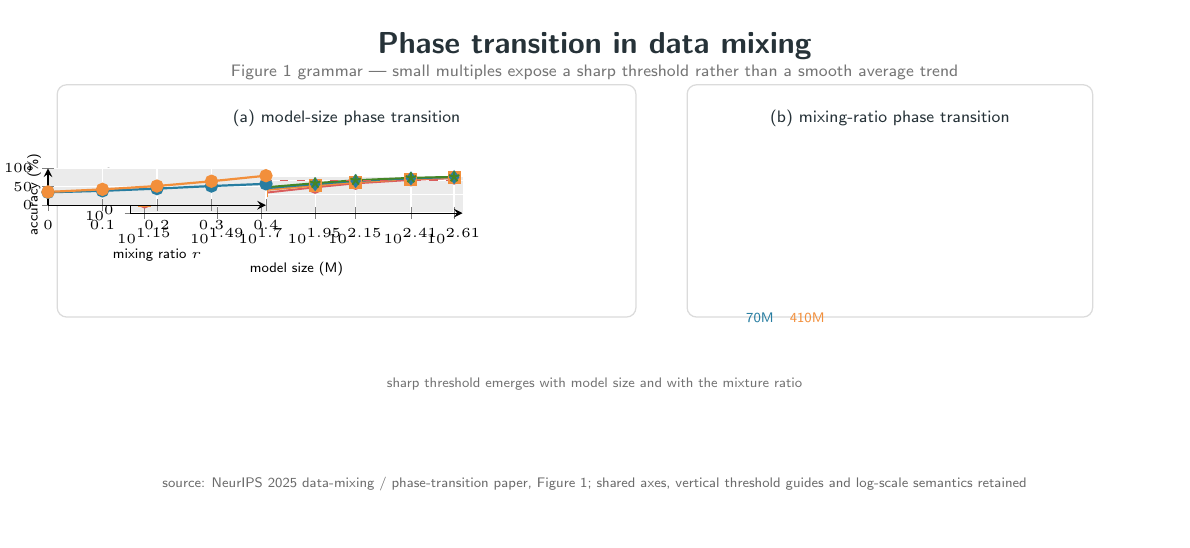
\begin{tikzpicture}[x=1cm,y=1cm]
\path[use as bounding box] (-.2,-4.0) rectangle (14.2,2.25);
\node[exact title,text=ptink] at (7,2.02) {Phase transition in data mixing};
\node[exact subtitle,text=black!54] at (7,1.68) {Figure 1 grammar — small multiples expose a sharp threshold rather than a smooth average trend};
\node[panel,minimum width=7.35cm,minimum height=2.95cm] at (3.85,.05) {};
\node[exact label,text=ptink] at (3.85,1.1) {(a) model-size phase transition};
\begin{axis}[at={(.95,-1.03)},width=5.8cm,height=2.05cm,xmode=log,ymode=log,xmin=12,xmax=450,ymin=1,ymax=100,axis lines=left,grid=major,grid style={white,line width=.45pt},major grid style={white},axis background/.style={fill=black!8},xtick={14,31,50,90,140,256,410},ytick={1,10,60,100},tick label style={font=\fontsize{4.1}{4.8}\selectfont},label style={font=\fontsize{4.6}{5}\selectfont},xlabel={model size (M)},ylabel={accuracy (\%)}]
\addplot[ptred,mark=*,line width=.7pt] coordinates {(14,4)(31,8)(50,12)(90,25)(140,41)(256,63)(410,79)};\addplot[ptorange,mark=square*,line width=.7pt] coordinates {(14,5)(31,10)(50,17)(90,31)(140,48)(256,70)(410,84)};\addplot[ptblue,mark=diamond*,line width=.7pt] coordinates {(14,6)(31,12)(50,21)(90,37)(140,55)(256,76)(410,89)};\addplot[ptgreen!80!black,mark=star,line width=.7pt] coordinates {(14,7)(31,14)(50,24)(90,42)(140,61)(256,82)(410,93)};\draw[ptred,dashed] (axis cs:12,60) -- (axis cs:450,60);\node[metric,text=ptred] at (axis cs:20,67) {60\% threshold};\end{axis}
\node[panel,minimum width=5.15cm,minimum height=2.95cm] at (10.75,.05) {};
\node[exact label,text=ptink] at (10.75,1.1) {(b) mixing-ratio phase transition};
\begin{axis}[at={(8.35,-1.03)},width=4.35cm,height=2.05cm,xmin=0,xmax=.4,ymin=0,ymax=100,axis lines=left,grid=major,grid style={white,line width=.45pt},axis background/.style={fill=black!8},xtick={0,.1,.2,.3,.4},ytick={0,50,100},tick label style={font=\fontsize{4.1}{4.8}\selectfont},label style={font=\fontsize{4.6}{5}\selectfont},xlabel={mixing ratio \(r\)},ylabel={accuracy}]
\addplot[ptblue,mark=*,line width=.8pt] coordinates {(0,35)(.1,39)(.2,45)(.3,52)(.4,58)};\addplot[ptorange,mark=*,line width=.8pt] coordinates {(0,36)(.1,43)(.2,52)(.3,65)(.4,80)};\end{axis}
\node[exact tiny,text=ptblue] at (9.1,-1.43) {70M};\node[exact tiny,text=ptorange] at (9.7,-1.43) {410M};
\node[exact tiny,text=black!55] at (7,-2.28) {sharp threshold emerges with model size and with the mixture ratio};
\node[exact tiny,text=black!58] at (7,-3.55) {source: NeurIPS 2025 data-mixing / phase-transition paper, Figure 1; shared axes, vertical threshold guides and log-scale semantics retained};
\end{tikzpicture}\end{document}
